\section{Models of Decision Support Considered}

This simulation project can be classified under multiple decision support model categories, as it touches upon different aspects of decision-making processes. Here's how the project fits into each of the categories:

\begin{enumerate}
    \item \textbf{Descriptive}

      This simulation contains a strong descriptive component.    
      During the initial stages, the agents are trained using DRL algorithms, and their behaviors are observed and recorded in a baseline scenario. This phase is focused on describing and understanding how the autonomous agents make decisions (e.g., crossing order, speed adjustment) based on the environment they are exposed to. The descriptive element helps us analyze how agents behave without interference and forms the basis for comparison with later stages.
      
    \item \textbf{Normative}

          This simulation implicitly contains a normative aspect.
      The desired outcomes for autonomous vehicle behavior (e.g., maximizing traffic flow while minimizing collisions) are rooted in optimal decision-making criteria. Although the project does not directly implement normative models, the success criteria for the agents—safe and efficient decision-making—are benchmarks derived from an ideal (normative) vision of how the system should behave in various traffic conditions.
      
    \item \textbf{Predictive}

          The simulation can be seen as predictive in its later stages.
      After training the agents, one of the goals is to predict how the multi-agent system (MAS) will perform under different traffic fluxes and lane configurations. The project aims to simulate a variety of scenarios (perturbations) and observe how the agents adapt. Through this, the system’s future performance in unseen scenarios can be forecast, making predictive modeling a key aspect of the evaluation.
      
    \item \textbf{Prescriptive}

          The simulation has a prescriptive element.
      The goal of DRL in this context is to prescribe optimal actions to agents in real-time traffic scenarios. By learning policies that guide the agents' decisions (e.g., what crossing order to take, when to accelerate or decelerate), the system effectively prescribes the best possible actions to optimize traffic flow and minimize collision risk. As the agents are trained to follow the best course of action in specific conditions, the project fits well within the prescriptive decision support model.
      
    \item \textbf{Speculative}

          The simulation could involve some speculative modeling, though this is not a primary focus.
      Testing agent performance in hypothetical situations would fall under this category, helping assess how flexible and adaptive the MAS is. However, speculative modeling is a minor aspect, as the primary focus is on concrete variations in traffic and lane configurations.
      
\end{enumerate}

Based on these observations, the primary classification of this simulation project would be \textbf{descriptive}, \textbf{predictive}, and \textbf{prescriptive}, as it involves understanding current decision-making, predicting agent behaviors under different conditions, and prescribing optimal actions for traffic optimization and safety.

Normative models are more implicit, serving as ideal benchmarks, while speculative elements might arise if the project explores hypothetical or extreme scenarios.

In addition to the decision support model categories, the simulation model can be classified as:

      \textbf{Dynamic}: The model evolves over time as agents continuously interact with the environment, make decisions, and adapt to changing conditions at road intersections. The system state changes as traffic flows and lane configurations adjust.
      
      \textbf{Stochastic}: The simulation includes elements of randomness, such as variations in traffic flow, vehicle arrival patterns, and potential uncertainties in agent behavior. This introduces probabilistic outcomes and variability across different simulation runs.
      
      \textbf{Discrete}: The model operates in discrete time steps, where the agents' actions (e.g., crossing intersections, adjusting speed) are evaluated at specific intervals. Each decision is made at distinct time points, typical in agent-based simulations where agent behaviors are updated step-by-step.
      
These classifications emphasize the dynamic, probabilistic, and step-wise nature of this agent-based simulation, where individual agents make decisions over time.

\section{The System as an Agent-Based Simulation}

As an \textbf{agent-based simulation}, this simulation's behavior emerges from the interactions of its individual agents, our autonomous vehicles. These vehicles represent entities capable of perceiving the environment and adapting their actions accordingly.

\textbf{Environment Entities}

In this context, the primary entities of the system can be described as:

\begin{enumerate}
    
    \item \textbf{Autonomous Vehicles (Agents):}
    
          Each autonomous vehicle represents an agent in the simulation with decision-making capabilities. These vehicles are created, move around, change speed, and interact with other agents. They may enter and leave the system as they pass through the intersection.
          
          Attributes: Speed, position, direction, assigned policy (decision-making model), current lane.
          
          Resources they compete for: Road space, crossing priority, lanes.
          
    \item \textbf{Intersection (Road Infrastructure)}:
    
          The road intersection is a static entity but a key part of the system. It defines where vehicles meet and interact. Different types of lane configurations or intersection designs can be applied.
          
          Attributes: Number of lanes, intersection layout.
          
          Resources they compete for: Lane capacity (the number of vehicles that can use a lane or section of road at a time).
          
    \item \textbf{Traffic Flow:}
    
          Represents the overall movement of vehicles through the system. This is a dynamic entity in terms of the rate at which vehicles arrive at and depart from the intersection.
          
          Attributes: Arrival rate of vehicles, traffic density, vehicle types (e.g. vehicles, ego-vehicles).
          
          Resources they compete for: Access to the intersection, road segments.
          
    \item \textbf{Agent Policies (Decision-Making Models):}
    
          Each autonomous vehicle (agent) operates based on a decision-making policy (learned behavior from DRL). These policies guide how each vehicle responds to other vehicles and environmental factors.
          
          Attributes: Learned policy, decision rules, reward function (for reinforcement learning).
          
          Resources they compete for: Computational resources for decision-making (though implicit in the model), control over vehicle behavior.
\end{enumerate}

\textbf{System Variables}

Variables in the system represent pieces of information that reflect characteristics of the entire system, not of specific entities. These variables are either directly influenced by the system dynamics or serve as global parameters for the simulation.

\begin{enumerate}

    \item \textbf{Exogeneous Variables}
    \begin{enumerate}
        \item\textbf{Non-Controllable}
            \begin{enumerate}
          
            \item \textbf{Traffic Density (Arrival Rate of Vehicles):}
                Indicates the rate at which vehicles enter the simulation, typically measured as vehicles per time unit (e.g., vehicles per minute).
                
                Role: It influences system congestion and vehicle interactions at the intersection.
                
            \item \textbf{Intersection Configuration (Lane Layout):}
                Represents the structure of the intersection, such as the number of lanes or the presence of dedicated turn lanes.
                
                Role: Changes in this variable affect how vehicles maneuver and interact with each other.
            \end{enumerate}  

        \item \textbf{Controllable}  
            \begin{enumerate}
                \item \textbf{Number of Controlled Vehicles}:  
                Specifies the number of ego-vehicles that can be simultaneously managed by the agent's policy.  

                \item \textbf{Agent-Implemented Policy}:  
                Enables the definition of the agent's policy and algorithm for each simulation scenario.  
            \end{enumerate}

    \end{enumerate}

    \item \textbf{Endogeneous Variables}
    \begin{enumerate}
    \item \textbf{Controlled Vehicles Average Speed:}
          This is a system-level variable that measures on average, the vehicles speed when crossing the intersection.
          
          Role: It reflects the system's efficiency and can be used to assess the performance of different policies.

    \item \textbf{Collision Rate:}
          A key variable that reflects the number of collisions or near-collisions occurring in the system.
          
          Role: A measure of the system's safety, which influences the evaluation of agent decision-making policies.
          
    \item \textbf{System Throughput:}
          The number of vehicles successfully passing through the intersection over a given period.
          
          Role: A variable that reflects the overall efficiency and capacity of the system, indicating how well it handles different traffic conditions.
    \end{enumerate}
\end{enumerate}

\begin{figure}[H]
    \centering
    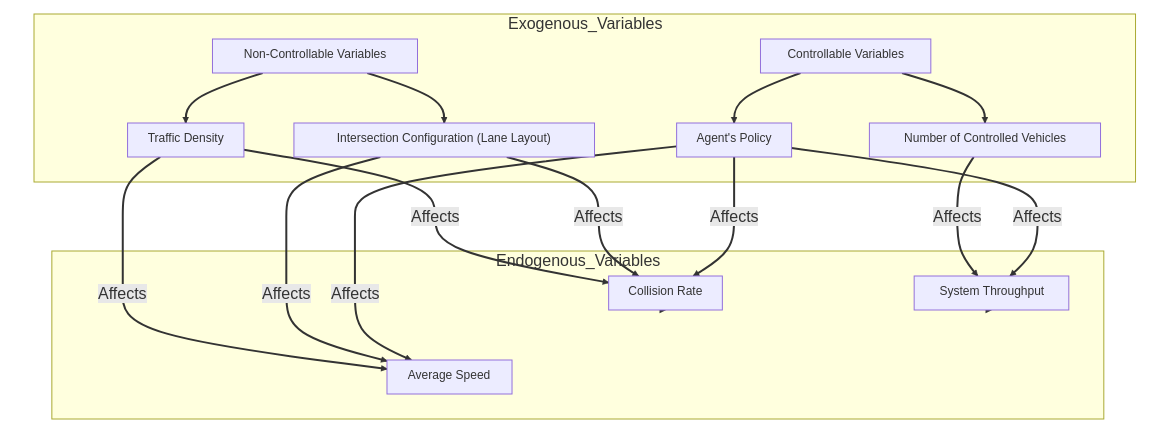
\includegraphics[height=0.25\textheight]{images/variables.png} 
    \caption{System Variables}
\end{figure}



\textbf{State of the System}:

The state of the system at any given time would include a collection of variables such as the number of vehicles in the system, traffic density, the intersection configuration, and the real-time position and speed of each vehicle. 

The state contains all the necessary information to describe the system's current dynamics and predict future behaviors.
      
These elements collectively define how the simulation operates, how decisions are made, and how the performance of the system is evaluated.



\section{Agent Training Algorithms and Policies to be Tested}

The simulation project will consist of three groups, each containing four agents trained using Deep Reinforcement Learning (DRL) techniques based on the \textbf{DQN} and \textbf{PPO} algorithms, employing different policies (\textit{MlpPolicy}, \textit{CnnPolicy}, and \textit{Social Attention Mechanisms}).

The behavior of these agents and their respective policies will be evaluated against a \textbf{Baseline Scenario}, where agents operate without any guiding policy and perform random actions.

\subsection{Training Algorithms}

\subsubsection{1.Deep Reinforcement Learning using DQN}

The Deep Q-Network (DQN) algorithm is a reinforcement learning approach designed to enable agents to learn optimal policies by estimating the value of action-state pairs~\cite{mnih2015dqn}. This is achieved by leveraging neural networks to approximate Q-values, which guide the agent's actions to maximize long-term rewards.

To understand DQN, we first define the concept of a Markov Decision Process (MDP). An MDP is characterized by states \(s\), actions \(a\), rewards \(r\), and transitions \(P(s' \mid s, a)\). The goal in an MDP is to maximize the cumulative reward (also known as the return) over time.

The Q-function represents the expected return of taking a specific action \(a\) in a given state \(s\), followed by an optimal sequence of actions:

\[
Q(s, a) = \mathbb{E} \left[ r_t + \gamma \max_{a'} Q(s_{t+1}, a') \mid s_t = s, a_t = a \right]
\]

Here:
- \(Q(s, a)\) is the value of taking action \(a\) in state \(s\),
- \(r_t\) is the immediate reward received,
- \(\gamma\) is the discount factor, where \(0 \leq \gamma \leq 1\), balancing the importance of immediate and future rewards.

The Q-function is recursively defined using the Bellman equation:

\[
Q(s, a) = r + \gamma \max_{a'} Q(s', a')
\]

In practice, DQN approximates the Q-function using a deep neural network parameterized by \(\theta\):

\[
Q(s, a; \theta) \approx Q^*(s, a)
\]

where \(Q^*(s, a)\) represents the optimal Q-function. 

The neural network learns the parameters \(\theta\) by minimizing the difference between predicted and target Q-values.


\subsubsection{2.Deep Reinforcement Learning using PPO}

Proximal Policy Optimization (PPO) is a reinforcement learning algorithm that aims to improve the policy of an agent by balancing exploration and exploitation\cite{schulman2017ppo}. 
PPO achieves this by using a clipped objective function to prevent large policy updates, ensuring stable learning.

\textbf{Policy Function}

The policy function \(\pi_\theta(a \mid s)\) defines the probability of taking action \(a\) in state \(s\) according to the policy parameters \(\theta\):

\[
\pi_\theta(a \mid s) = \mathbb{P}(a \mid s; \theta)
\]

Here, \(\theta\) parameterizes the policy network. In PPO, the goal is to maximize cumulative rewards while ensuring stability by limiting updates using a clipped objective function.

\textbf{PPO Objective Function}

The objective function used in PPO is a clipped surrogate objective, which aims to optimize the policy by maximizing the expected advantage, but with a constraint on the update size:

\[
L(\theta) = \mathbb{E}_t \left[ \min \left( r_t(\theta) A_t, \text{clip}(r_t(\theta), 1-\epsilon, 1+\epsilon) A_t \right) \right]
\]

Where:
- \(r_t(\theta)\) is the probability ratio between the new and old policy, defined as:

\[
r_t(\theta) = \frac{\pi_\theta(a_t \mid s_t)}{\pi_{\theta_{\text{old}}}(a_t \mid s_t)}
\]

- \(\epsilon\) is the clipping parameter, controlling how much the policy is allowed to change.
- \(A_t\) is the advantage estimate at time step \(t\), which measures how much better an action is compared to the average action.


\subsection{Agent Policies}

We will compare agents' behavior based on four distinct policies:

\begin{enumerate}
    \item\textbf{Baseline {No Policy}}

    \item\textbf{MlpPolicy (Multi-Layer Perceptron Policy)}
    
    The \textit{MlpPolicy} utilizes a multi-layer perceptron neural network to process environmental observations and make decisions. This policy focuses on key input features, such as speed, distance to other vehicles, and intersection layout, allowing agents to act based on their immediate surroundings.

    \textbf{Scenario}: Agents following the \textit{MlpPolicy} will navigate the intersection by leveraging their observed features, applying learned behaviors to respond effectively to dynamic traffic conditions.

    \textbf{Objective}: Assess the performance of \textit{MlpPolicy} agents in terms of efficiency (e.g., throughput, wait times) and safety (e.g., collision rates) compared to agents using other policies. Analyze the influence of input features on their decision-making processes.

    \item\textbf{CnnPolicy (Convolutional Neural Network Policy)}
    
    The \textit{CnnPolicy} employs convolutional neural networks to process visual and spatial data, making it particularly effective in scenarios where visual inputs (like grid representations of the intersection) are crucial for decision-making.

    \textbf{Scenario}: Agents using the \textit{CnnPolicy} will interpret complex visual representations of their environment, allowing them to make informed decisions regarding lane changes, merging, and crossing orders.

    \textbf{Objective}: Evaluate the performance of \textit{CnnPolicy} agents in diverse traffic patterns, focusing on their ability to recognize spatial configurations and respond appropriately to traffic dynamics.

    \item\textbf{Social Attention Mechanisms Policy}
    
    This policy integrates social attention mechanisms, allowing agents to observe and interpret the behaviors and intentions of nearby vehicles. 

Social Attention Mechanisms in Deep Reinforcement Learning (DRL) are inspired by how humans or animals interact within a social environment.
In the context of multi-agent systems, the idea is to integrate social information, allowing agents to pay attention to the behavior and 
intentions of other agents.\cite{sutton2018reinforcement}
This concept helps improve cooperation, communication, and coordination between agents in environments where agents need to share space and interact with each other, such as autonomous vehicles in a traffic intersection.


\paragraph{Attention Mechanisms} 
In deep learning, attention mechanisms allow models to focus on important parts of the input data when making decisions, 
rather than processing everything equally\cite{vaswani2017attention}. 
This is especially useful in scenarios involving sequences or spatial relations, where certain elements might be more significant than others.

\paragraph{Social Attention Mechanisms} 
Social attention mechanisms focus on enabling agents to learn which other agents (or parts of the environment) are most relevant to their actions. 
In the case of DRL with DQN (Deep Q-Network), these mechanisms could take into account the actions and states of surrounding agents when determining a given agent's own actions. 
Essentially, the agent learns a social context that goes beyond its immediate environment\cite{jiang2018learning}.


\paragraph{State Representation with Social Attention} 
In a multi-agent setting, an agent’s state at time $t$, $s_t$, may include not only its own environment but also the states of surrounding agents. Let the state of agent $i$ be represented as $s_i(t)$, and the full state of the environment, including information from other agents, can be written as:
\[
s_t = \{s_i(t), s_{-i}(t)\}
\]
where $s_{-i}(t)$ represents the states of all other agents in the environment at time $t$\cite{mnih2015dqn}.

\paragraph{Social Attention Weights} 
A key idea in social attention is to compute attention weights that determine how much focus an agent should place on each neighboring agent. Let $\alpha_i$ be the attention weight for agent $i$. These weights are learned through a neural network that estimates the importance of each neighboring agent's state in the context of the decision-making process. A common approach is to use a weighted sum, where each agent’s state is weighted according to its relevance:
\[
\tilde{s}_t = \sum_{i \in N} \alpha_i s_i(t)
\]
where $N$ is the set of neighboring agents, and $\alpha_i$ is the attention weight for agent $i$. This process enables each agent to selectively attend to those agents whose states or actions influence its own behavior.

\paragraph{Modifying the Q-Function with Attention} 
The standard DQN Q-function estimates the expected return for each action given a state $s_t$. With the incorporation of social attention, we modify the Q-function to account for the social context:
\[
Q(s_t, a_t) = \mathbb{E}\left[r_t + \gamma \max_{a_{t+1}} Q(s_{t+1}, a_{t+1}; \theta) \mid s_t, a_t\right]
\]
where $s_t$ now includes the social context $\tilde{s}_t$, representing the attention-weighted sum of the agent’s own state and the states of the other agents. The DQN network then estimates the Q-values with this enriched state.

\paragraph{Multi-Head Attention Implementation}
The attention mechanism utilizes multiple heads to compute context-sensitive embeddings, allowing the model to attend to different aspects of the input simultaneously. Each head processes the embeddings independently and outputs its own context-aware representation. The outputs from all heads are concatenated and projected to form the final embedding. The attention computation for each head is given by\cite{DBLP}:
\[
\text{output} = \sigma \left( \frac{Q K^T}{\sqrt{d_k}} \right) V
\]
where:
\[
Q = L_q(e_0), \; K = L_k(e_i), \; V = L_v(e_i)
\]

In these equations:
- $e_i$ denotes the encoded state of vehicle $i$, while $e_0$ corresponds to the ego-vehicle
- $K$ (keys) represents descriptive features of surrounding vehicles
- $V$ (values) contains the embedded features used to compute the final output
- $L_q$, $L_k$, $L_v$ are shared linear projections applied to all vehicles' embeddings
- $\sigma$ is the softmax activation, normalizing attention scores across all vehicles
- $d_k$ represents the dimension of the key embeddings

The ego-vehicle query $Q$ interacts with keys $K$ to compute attention weights, prioritizing vehicles that are most relevant to the ego-vehicle's current context. This results in a weighted combination of values $V$. The outputs from each head are aggregated and passed through a linear layer to produce the final representation.


    This approach helps agents develop cooperative strategies and optimize their interactions with other vehicles. 
    The attention architecture was introduced to enable neural networks to discover inter-dependencies within a variable number of inputs\cite{vaswani2017attention}.



    
    \textbf{Scenario}: Agents utilizing this policy will actively monitor the behavior of surrounding vehicles, adapting their actions based on predicted movements and intentions of others.

    \textbf{Objective}: Investigate the effectiveness of social attention in enhancing cooperation among agents, potentially leading to improved traffic flow and reduced collision rates. 
    Compare the performance of agents using Social Attention Mechanisms against those following other policies to assess their overall effectiveness in a multi-agent environment.
\end{enumerate}


\section{Testing Framework for Operation Policies (Scenarios)}

\begin{enumerate}
    \item \textbf{Experimental Scenarios:} Each policy will be tested under various conditions, such as:
    \begin{itemize}
        \item \textbf{High Traffic Density:} Increased number of vehicles entering the intersection simultaneously.
        \item \textbf{Low Traffic Density:} Sparse vehicle presence to evaluate agent behavior in less congested environments.
    \end{itemize}
    \item \textbf{Group Configuration:} Each group, consisting of four agents using the same policy, will be tested in each scenario. This allows for direct comparisons between the different policies under identical traffic conditions.
    \item \textbf{Performance Metrics:}
    \begin{enumerate}
        \item \textbf{Efficiency:} Metrics such as throughput (vehicles per time unit), and average speed of agents.
        \item \textbf{Safety:} Collision rates, near-misses, and compliance with traffic rules.
        \item \textbf{Adaptability:} How well agents generalize their learned behaviors to new traffic scenarios (e.g., changes in traffic density, lane configurations).
    \end{enumerate}
\end{enumerate}


\section{Global Key Performance Indicators (KPI)}

The following Key Performance Indicators (KPIs) and decision criteria will be used to effectively assess the performance and effectiveness of the operational policies:

\begin{enumerate}
    \item \textbf{Traffic Flow Efficiency}
    \begin{itemize}
        \item \textbf{Metric:} Average vehicle throughput (Arrived vehicles per test episode)
        \item This metric measures how well the intersection handles traffic. A higher throughput indicates that the system is efficiently managing vehicle movement.
    \end{itemize}
    
    \item \textbf{Safety Metrics}
    \begin{itemize}
        \item \textbf{Metric:} Collision rate (Average number of collisions per test episode)
        \item This is a crucial indicator of how safe the intersection is for autonomous vehicles. Reducing collisions is a primary goal for any traffic management system.
    \end{itemize}
    
    \item \textbf{Adaptability to Varying Traffic Conditions}
    \begin{itemize}
        \item \textbf{Metric:} Performance variance (e.g., comparing metrics like wait times and throughput under different traffic densities)
        \item This evaluates how well agents can adjust their behavior to different traffic conditions, ensuring the system's flexibility in dynamic environments.
    \end{itemize}
\end{enumerate}

